\chapter{从花到果}\label{ch:g5:flower-to-fruit}

\Cref{ch:g3:flowers-fruits-seeds}中看到樱花
变成樱桃，并留下一个悬而未决的问题：当一粒\omterm{def:g3:flowers-fruits-seeds:parts}{花粉}落在\omterm{def:g3:flowers-fruits-seeds:parts}{雌蕊}上时，
\emph{究竟发生了什么}？
本学年，我们借助\cref{ch:g4:animal-reproduction}中的\omterm{def:g5:flower-to-fruit:steps}{受精}概念，
以及\cref{ch:g5:first-look-at-cells}中的\omterm{def:g5:first-look-at-cells:cell}{细胞}知识，
可以深入探究花的运作机制。

\section{花有雄性和雌性部分}

\begin{proposition}[花的两种作用集于一身]\label{prop:g5:flower-to-fruit:roles}
被子\omterm{def:g1:plants-around-us:plant}{植物}的繁殖属于\emph{有性}
生殖，完全符合
\cref{def:g4:animal-reproduction:sexual}中的含义——而且多数
花同时兼具两种作用：
\begin{itemize}
  \item \emph{\omterm{def:g3:flowers-fruits-seeds:parts}{雄蕊}}是\omterm{def:g4:animal-reproduction:sexual}{雄性}部分：每一粒
        \emph{\omterm{def:g3:flowers-fruits-seeds:parts}{花粉}}携带\omterm{def:g1:plants-around-us:plant}{植物}的\omterm{def:g4:animal-reproduction:sexual}{雄性}
        生殖\omterm{def:g5:first-look-at-cells:cell}{细胞}；
  \item \emph{\omterm{def:g3:flowers-fruits-seeds:parts}{雌蕊}}是\omterm{def:g4:animal-reproduction:sexual}{雌性}部分：其内部深处
        藏有\emph{胚珠}\index{胚珠}，每个\omterm{prop:g5:flower-to-fruit:roles}{胚珠}内含一个
        \omterm{def:g4:animal-reproduction:sexual}{卵细胞}。
\end{itemize}
“未来的\omterm{def:g2:from-seed-to-plant:seed}{种子}”，即
\cref{def:g3:flowers-fruits-seeds:parts}中所说的，
如今有了真正的名字：\omterm{prop:g5:flower-to-fruit:roles}{胚珠}，正等待\omterm{def:g5:flower-to-fruit:steps}{受精}。
\end{proposition}
\admitted

\begin{remark}[与动物的方案相同]\label{rem:g5:flower-to-fruit:sameplan}
\omterm{def:g4:animal-reproduction:sexual}{雄性}\omterm{def:g5:first-look-at-cells:cell}{细胞}、\omterm{def:g4:animal-reproduction:sexual}{卵细胞}、\omterm{def:g5:flower-to-fruit:steps}{受精}等说法，
\cref{ch:g4:animal-reproduction}中的词汇可直接套用。
\omterm{prop:g5:first-look-at-cells:principle}{生命的统一性}再次体现
（见\cref{prop:g5:first-look-at-cells:principle}）——雏菊
和海豚都依据同一基本方案繁殖，
尽管其构造看上去差异很大。
\end{remark}

\section{先传粉，后受精}

\begin{definition}[两个步骤]\label{def:g5:flower-to-fruit:steps}
形成\omterm{def:g2:from-seed-to-plant:seed}{种子}需要两个不同的步骤：
\begin{enumerate}
  \item \emph{传粉}\index{传粉}：一粒\omterm{def:g3:flowers-fruits-seeds:parts}{花粉}
        从\omterm{def:g3:flowers-fruits-seeds:parts}{雄蕊}传送到\omterm{def:g3:flowers-fruits-seeds:parts}{雌蕊}顶端——
        借助\omterm{prop:g3:sorting-living-things:groups}{昆虫}
        （见\cref{prop:g3:flowers-fruits-seeds:transform}）或借助
        风力；
  \item \emph{受精}\index{受精（植物）}：
        落下的\omterm{def:g3:flowers-fruits-seeds:parts}{花粉}粒长出一条细管，\emph{沿\omterm{def:g3:flowers-fruits-seeds:parts}{雌蕊}向下}
        延伸；经由这条管，\omterm{def:g4:animal-reproduction:sexual}{雄性}\omterm{def:g5:first-look-at-cells:cell}{细胞}抵达
        一个\omterm{prop:g5:flower-to-fruit:roles}{胚珠}，并与其\omterm{def:g4:animal-reproduction:sexual}{卵细胞}结合。
\end{enumerate}
传粉是旅程，受精是相遇。
\end{definition}

\begin{omfigure}
\begin{tikzpicture}
  \node[anchor=south west, inner sep=0] (img) at (0,0)
    {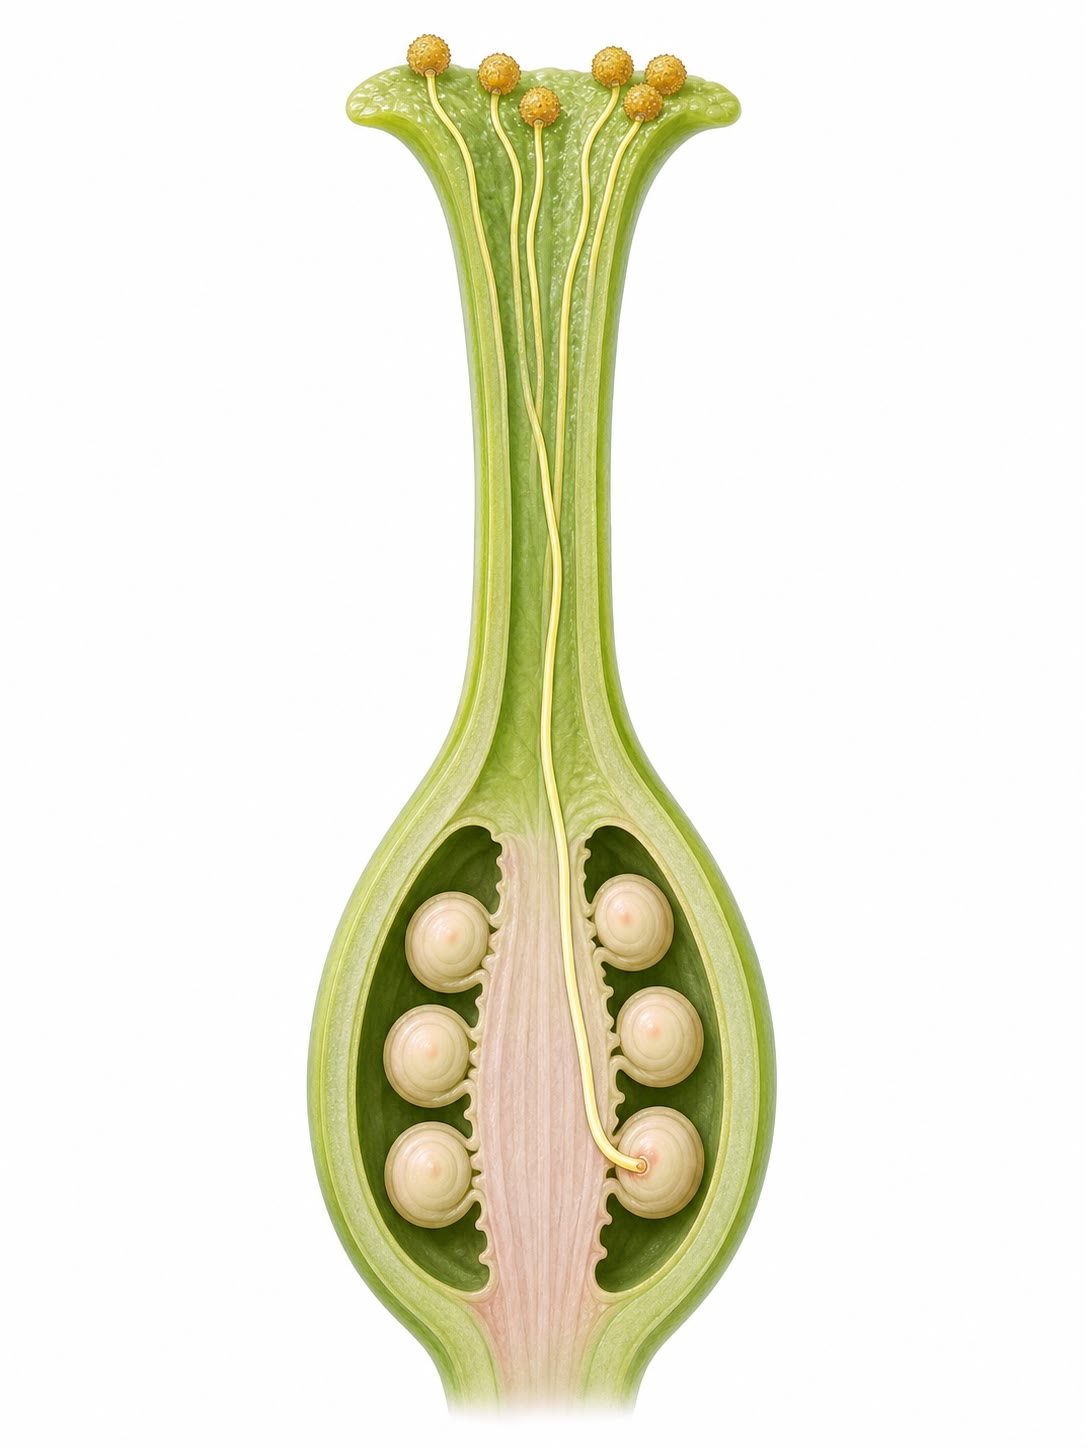
\includegraphics[width=0.42\linewidth]{images/book1/ai/fig-pistil-tube.jpg}};
  \begin{scope}[x={(img.south east)}, y={(img.north west)},
      every node/.style={font=\small}]
    \draw[omProp, thick] (0.62,0.95) -- (0.80,0.97)
      node[right, align=left, omProp]
      {花粉落下：\\ 传粉};
    \draw[omProp, thick] (0.53,0.55) -- (0.78,0.60)
      node[right, align=left, omProp]
      {花粉管 \\ 向下生长};
    \draw[omDef, thick] (0.36,0.26) -- (-0.05,0.30)
      node[left, align=right, omDef]
      {胚珠，各含 \\ 一个卵细胞};
    \draw[omDef, thick] (0.62,0.15) -- (0.80,0.11)
      node[right, align=left, omDef]
      {雄性细胞抵达：\\ 受精};
  \end{scope}
\end{tikzpicture}

{\small \omterm{def:g3:flowers-fruits-seeds:parts}{雌蕊}内部：落下的\omterm{def:g3:flowers-fruits-seeds:parts}{花粉}粒长出\omterm{def:g3:flowers-fruits-seeds:parts}{花粉}管
向下延伸至\omterm{prop:g5:flower-to-fruit:roles}{胚珠}，\omterm{def:g5:flower-to-fruit:steps}{受精}发生在底部。}
\end{omfigure}

\begin{example}[为什么未传粉的花会凋落]\label{ex:g5:flower-to-fruit:unvisited}
\Cref{rem:g3:flowers-fruits-seeds:bees}中的果园规则，如今
有了其机制：没有访花，\omterm{def:g3:flowers-fruits-seeds:parts}{雌蕊}上便没有\omterm{def:g3:flowers-fruits-seeds:parts}{花粉}；
没有\omterm{def:g3:flowers-fruits-seeds:parts}{花粉}，就没有\omterm{def:g3:flowers-fruits-seeds:parts}{花粉}管，也就没有\omterm{def:g5:flower-to-fruit:steps}{受精}；未\omterm{def:g5:flower-to-fruit:steps}{受精}的花
整朵枯萎——\omterm{def:g3:flowers-fruits-seeds:parts}{雌蕊}不再膨大，也就没有樱桃。
缺失的那一步肉眼看不见，即\omterm{def:g5:first-look-at-cells:cell}{细胞}沿管道下行的旅程——
但七月里光秃的枝条已经足够明显了。
\end{example}

\section{受精之后：种子与果实}

\begin{proposition}[各部分的去向]\label{prop:g5:flower-to-fruit:becomes}
\omterm{def:g5:flower-to-fruit:steps}{受精}之后，
\cref{prop:g3:flowers-fruits-seeds:transform}中所述的转化
以更为精确的方式进行：
\begin{itemize}
  \item 每个\emph{\omterm{def:g5:flower-to-fruit:steps}{受精}\omterm{prop:g5:flower-to-fruit:roles}{胚珠}}发育成
        \emph{\omterm{def:g2:from-seed-to-plant:seed}{种子}}——其中的幼小植株
        （见\cref{def:g2:from-seed-to-plant:seed}）由
        \omterm{def:g5:flower-to-fruit:steps}{受精}卵发育而来，正如\omterm{def:g1:animals-around-us:animal}{动物}
        由自身的\omterm{def:g5:flower-to-fruit:steps}{受精}卵长成
        （见\cref{ex:g5:first-look-at-cells:one}）；
  \item 包围它们的\emph{\omterm{def:g3:flowers-fruits-seeds:parts}{雌蕊}}膨大为
        \emph{\omterm{prop:g3:flowers-fruits-seeds:transform}{果实}}；
  \item \omterm{def:g3:flowers-fruits-seeds:parts}{花瓣}和\omterm{def:g3:flowers-fruits-seeds:parts}{雄蕊}完成使命后，枯萎
        脱落。
\end{itemize}
\end{proposition}
\admitted

\begin{example}[数苹果籽]\label{ex:g5:flower-to-fruit:pips}
把苹果横切开：有五个小房间，每间里有几粒
苹果籽。每粒籽对应一个被\omterm{def:g3:flowers-fruits-seeds:parts}{花粉}管
到达过的\omterm{prop:g5:flower-to-fruit:roles}{胚珠}。一侧空房间多、歪斜的苹果，
说明花的\omterm{def:g5:flower-to-fruit:steps}{传粉}不足——落上的\omterm{def:g3:flowers-fruits-seeds:parts}{花粉}粒太少，
不够使所有\omterm{prop:g5:flower-to-fruit:roles}{胚珠}\omterm{def:g5:flower-to-fruit:steps}{受精}，\omterm{prop:g3:flowers-fruits-seeds:transform}{果实}因而发育不均。
\end{example}

\begin{omfigure}
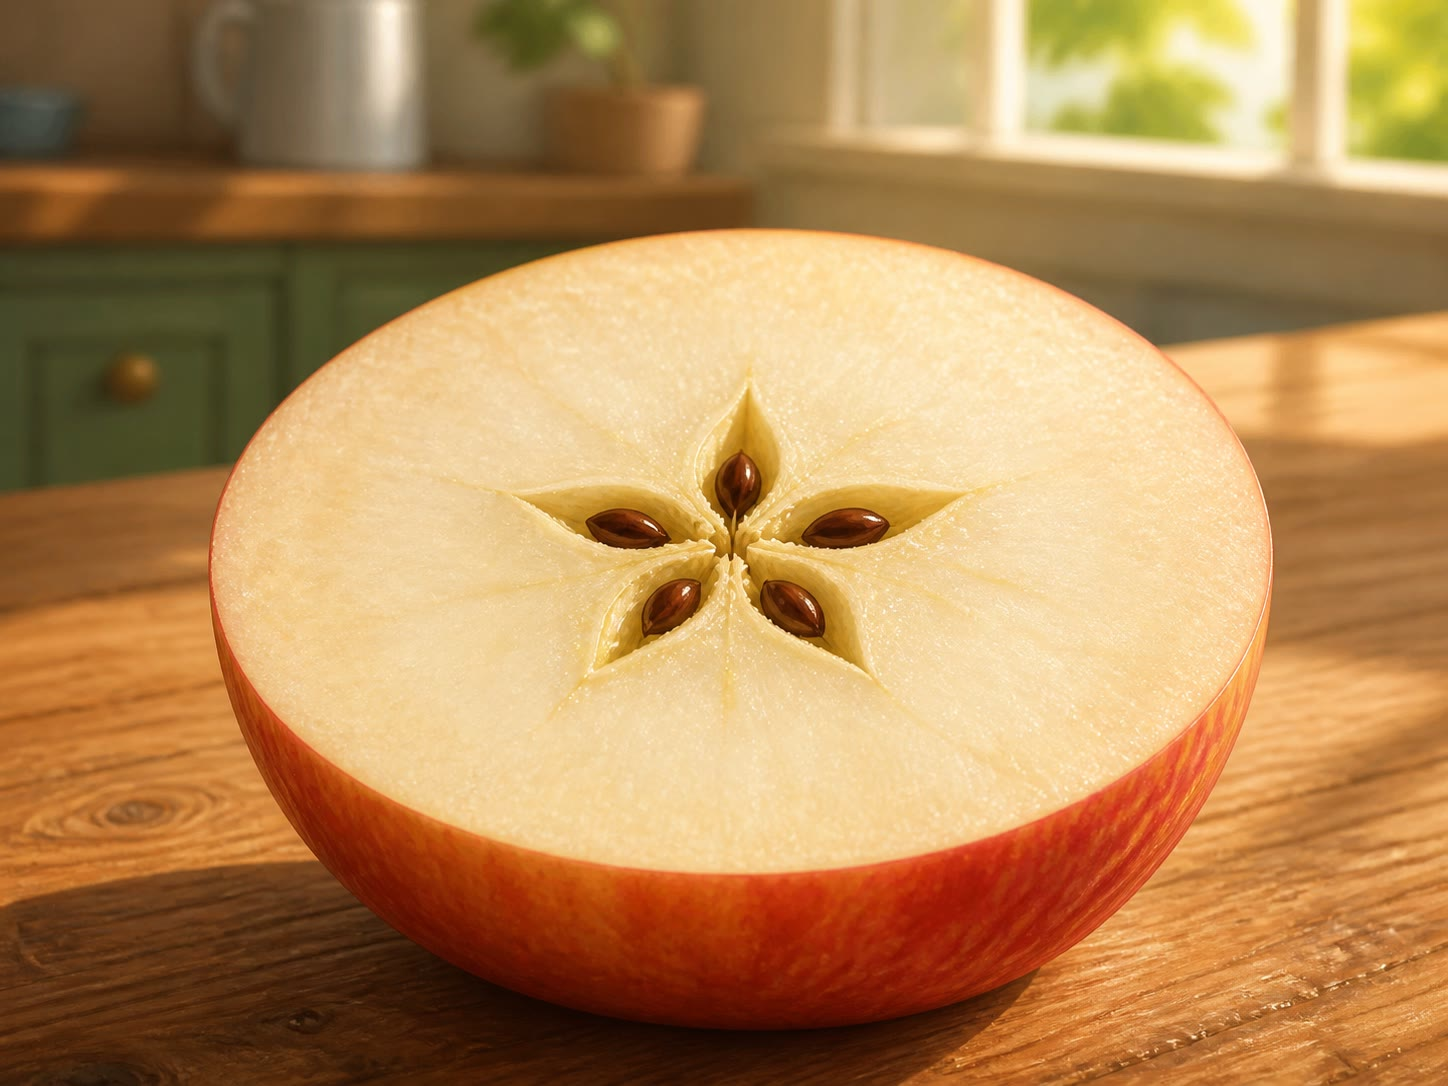
\includegraphics[width=0.56\linewidth]{images/book1/ai/g5-flower-applepips.jpg}

{\small 横切开的苹果：五个房间呈星形排列，
其中是苹果籽——每粒籽对应一个被\omterm{def:g3:flowers-fruits-seeds:parts}{花粉}管
到达过的\omterm{prop:g5:flower-to-fruit:roles}{胚珠}。}
\end{omfigure}

\begin{example}[风传花粉]\label{ex:g5:flower-to-fruit:wind}
草、小麦和榛树没有\omterm{def:g3:flowers-fruits-seeds:parts}{花瓣}、没有香味、没有
花蜜——没有东西可以提供给访客。它们的\omterm{def:g3:flowers-fruits-seeds:parts}{花粉}借
\emph{风}传播：大量产生，细如尘埃，
被抛入空中，落到哪里全凭运气。这一策略以
精确换数量——与
\cref{rem:g4:plants-without-seeds:sporeseed}中的\omterm{def:g4:plants-without-seeds:spore}{孢子}云思路相同，只是换成了\omterm{def:g3:flowers-fruits-seeds:parts}{花粉}。
（顺带一提，正是这种飘浮的\omterm{def:g3:flowers-fruits-seeds:parts}{花粉}，
使六月里患\omterm{def:g3:flowers-fruits-seeds:parts}{花粉}过敏的人鼻子发痒。）
\end{example}

\begin{method}[诊断不结果的植物]\label{met:g5:flower-to-fruit:diagnose}
一株\omterm{def:g1:plants-around-us:plant}{植物}开花很好，却不结果。按顺序询问：
\begin{enumerate}
  \item \omterm{def:g5:flower-to-fruit:steps}{传粉}者是否到达了它？（室内、套网、附近无\omterm{prop:g3:sorting-living-things:groups}{昆虫}、
        开花期的几周寒冷多雨？）
  \item 若没有，则人工授粉：先用软毛刷碰触
        一朵花的\omterm{def:g3:flowers-fruits-seeds:parts}{雄蕊}，再碰触
        另一朵花的\omterm{def:g3:flowers-fruits-seeds:parts}{雌蕊}；
  \item 霜冻或损伤是否在
        \omterm{prop:g5:flower-to-fruit:roles}{胚珠}\omterm{def:g5:flower-to-fruit:steps}{受精}之前就杀死了\omterm{def:g1:plants-around-us:parts}{花朵}
        （见\cref{exo:g3:flowers-fruits-seeds:9}）？
  \item 若此时\omterm{prop:g3:flowers-fruits-seeds:transform}{果实}开始结出，说明\omterm{def:g1:plants-around-us:plant}{植物}的机制完好，
        只是第 1 步的\omterm{def:g5:flower-to-fruit:steps}{传粉}失败了。
\end{enumerate}
\end{method}

\section{练习}

\begin{exercise}[$\star$]\label{exo:g5:flower-to-fruit:1}
花的哪一部分是\omterm{def:g4:animal-reproduction:sexual}{雄性}的，它产生什么？
哪一部分是\omterm{def:g4:animal-reproduction:sexual}{雌性}的？它里面有什么？
\end{exercise}

\begin{exercise}[$\star$]\label{exo:g5:flower-to-fruit:2}
给出\omterm{def:g5:flower-to-fruit:steps}{传粉}和\omterm{def:g5:flower-to-fruit:steps}{受精}的定义，并说明
二者中哪个先发生。
\end{exercise}

\begin{exercise}[$\star$]\label{exo:g5:flower-to-fruit:3}
描述一粒\omterm{def:g3:flowers-fruits-seeds:parts}{花粉}从\omterm{def:g3:flowers-fruits-seeds:parts}{雄蕊}到\omterm{def:g4:animal-reproduction:sexual}{卵
细胞}的过程，分四步写出。
\end{exercise}

\begin{exercise}[$\star$]\label{exo:g5:flower-to-fruit:4}
\omterm{def:g5:flower-to-fruit:steps}{受精}之后，每个\omterm{def:g5:flower-to-fruit:steps}{受精}的\omterm{prop:g5:flower-to-fruit:roles}{胚珠}会发育成什么？
\omterm{def:g3:flowers-fruits-seeds:parts}{雌蕊}会变成什么？\omterm{def:g3:flowers-fruits-seeds:parts}{花瓣}又会怎样？
\end{exercise}

\begin{exercise}[$\star$]\label{exo:g5:flower-to-fruit:5}
用本章的术语，每粒苹果籽是什么？
一侧空房间多、歪斜的苹果说明了什么？
\end{exercise}

\begin{exercise}[$\star$]\label{exo:g5:flower-to-fruit:6}
草和榛树在没有\omterm{def:g3:flowers-fruits-seeds:parts}{花瓣}、香味
或花蜜的情况下如何\omterm{def:g5:flower-to-fruit:steps}{传粉}？这种方式付出了什么代价？
\end{exercise}

\begin{exercise}[$\star$]\label{exo:g5:flower-to-fruit:7}
为什么没有\omterm{prop:g3:sorting-living-things:groups}{昆虫}光顾过的花通常
不结果？指出缺少的那一步。
\end{exercise}

\begin{exercise}[$\star$]\label{exo:g5:flower-to-fruit:8}
动手试一试（用开花的阳台或窗台\omterm{def:g1:plants-around-us:plant}{植物}）：
用软毛刷为两朵花人工授粉（做法见
\cref{met:g5:flower-to-fruit:diagnose}），并用
线绳为它们做记号。这些做过记号的花，结果
是否比其他花更多？
\end{exercise}

\begin{exercise}[$\star\star$]\label{exo:g5:flower-to-fruit:9}
列出\omterm{def:g1:plants-around-us:plant}{植物}与\omterm{def:g1:animals-around-us:animal}{动物}繁殖之间的相似之处：
\omterm{def:g4:animal-reproduction:sexual}{雄性}\omterm{def:g5:first-look-at-cells:cell}{细胞}、\omterm{def:g4:animal-reproduction:sexual}{卵细胞}、\omterm{def:g5:flower-to-fruit:steps}{受精}，以及新个体的
第一个\omterm{def:g5:first-look-at-cells:cell}{细胞}。以花为例，每一项分别位于
哪里？
\end{exercise}

\begin{exercise}[$\star\star$]\label{exo:g5:flower-to-fruit:10}
一位樱桃种植者的春季寒冷多雨：蜜蜂
连续两周几乎不飞出，虽然没有霜冻，树木
却开花很盛。请预测七月的收成，并用
\cref{def:g5:flower-to-fruit:steps}解释原因。
\end{exercise}

\begin{exercise}[$\star\star\star$]\label{exo:g5:flower-to-fruit:11}
一位温室番茄种植者在室内放入一箱熊蜂，
尽管从密闭温室中无法接触到外面的花。请运用本章内容，
准确说明熊蜂提供的是什么服务——以及为何
吹过植株的风扇能部分替代它们，
为番茄授粉（番茄\omterm{def:g3:flowers-fruits-seeds:parts}{花粉}会被震落），而对樱桃树
则做不到。
做不到。
\end{exercise}
